
\section{Results and Discussion}
\label{sec:Results}

In order to evaluate the impacts of different components of our hybrid system, a series of experiments are conducted. Firstly, we quantitatively analyze the reconstruction quality using a ground-truth model scanned by an accurate Lidar scanner.
Secondly, we show the reconstructed models of human bodies under different pose to demonstrate the robustness of our method.


%\noindent\textbf{Camera Calibration Accuracy.}
%The reprojection error of the proposed global calibration method is the smaller \xj{smallest?} among different methods, which proves that the global optimization is quite effective.
%Although the registration step makes the model closer to the ground truth, it leads to bigger reprojection error. That is because the aim of the registration step is to minimize the error caused by the inaccurate depth estimation, but not to optimize the camera parameters.


\noindent\textbf{Reconstruction Quality.}
%\xj{Explain why do you need this experiment.}
The final goal of our system is to achieve a high-quality reconstruction model, we quantitatively compare the results reconstructed by different methods.
%
We generate a ground-truth model by scanning a plaster model of a human head using a 3D laser scanner with the scanning error smaller than 0.04 mm within one meter.
%
The model is placed in our multi-camera system and the RGB and depth images of it can be obtained.
%We consider the accurate mesh as the ground truth and compare it with the reconstructed 3D model using different methods.
We compute the L2 distances of the fused point clouds to the ground-truth mesh for different variants of our method.
For each point $\vb{p}$ in the reconstructed point cloud, we search for its nearest point $\vb{q}$ on the mesh, and compute the distance $\|\vb{p}-\vb{q}\|$.
%
We divide the distance from 0 mm to 40 mm into 16 intervals and count the total number of the points in each interval. We show the distribution and the error bars of the distances using various methods in Figure~\ref{fig:histogram}. As we can see, the number of the points with small distance increases obviously after the optimization and registration step we proposed. Meanwhile, the reconstructed model combining the global calibration and registration has the smallest error, which proves that it can achieve a high-quality model.
\begin{figure}[ht]
%
\begin{minipage}[c]{0.49\linewidth}
  \centering
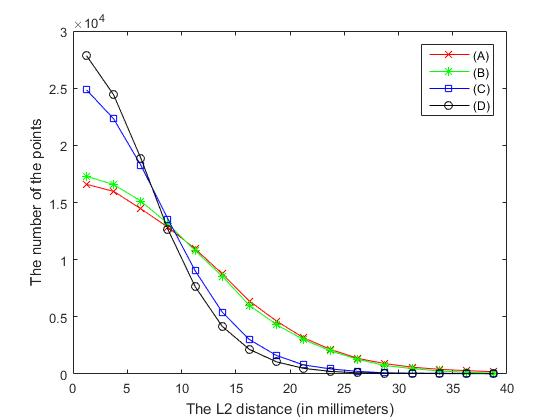
\includegraphics[width=4.4cm]{image/distribution.jpg}

  \centerline{(a)}\medskip
\end{minipage}
\hfill
\begin{minipage}[c]{0.49\linewidth}
  \centering
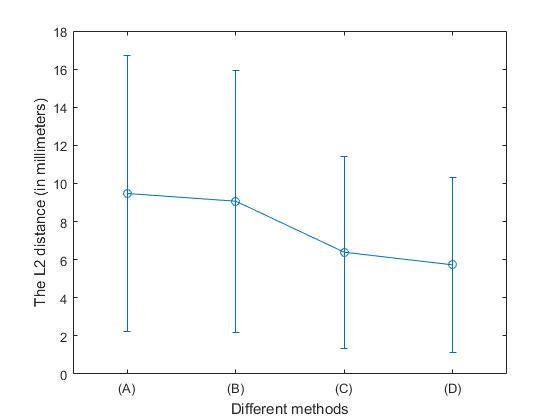
\includegraphics[width=4.4cm]{image/errorbar.jpg}

  \centerline{(b)}\medskip
\end{minipage}
%
\caption{The distribution and error bars of the L2 distances of the point cloud reconstructed using different methods to the ground truth. (A) results by Kalibr~\cite{Maye2013Self}, (B) results by Kalibr~\cite{Maye2013Self} with our registration step, (C) results by our global calibration method, (D) results by our integrated method.}
\label{fig:histogram}
\end{figure}


\noindent \textbf{More Reconstructed Models.}
%

\begin{figure*}[htbp]
  \centering
\subfigure[]{
\begin{minipage}[c]{.22\linewidth}
\centering
  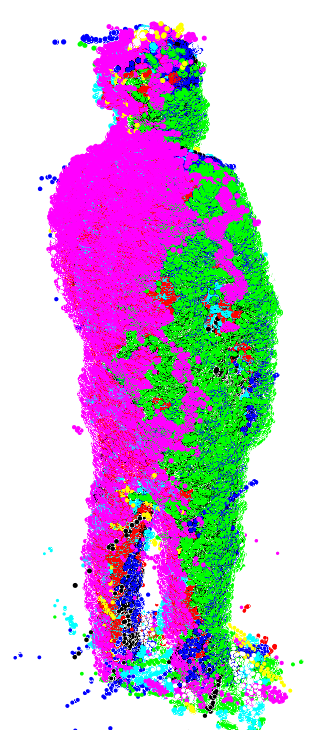
\includegraphics[width=2.5cm]{image/pc_1.png}
\end{minipage}
}%
\subfigure[]{
\begin{minipage}[c]{.22\linewidth}
\centering
  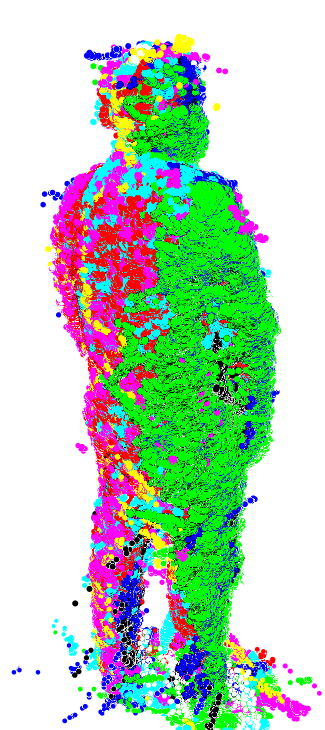
\includegraphics[width=2.5cm]{image/pc_2.png}
\end{minipage}
}
\subfigure[]{
\begin{minipage}[c]{.22\linewidth}
\centering
  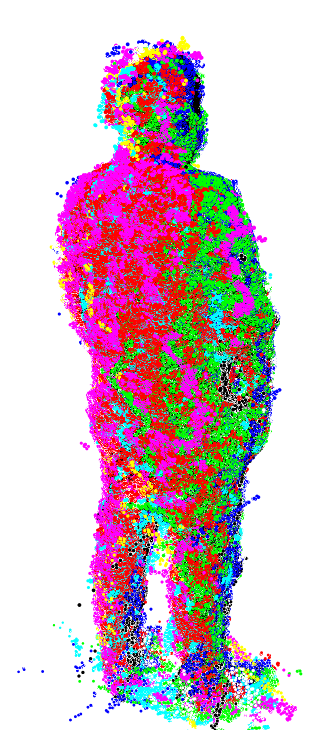
\includegraphics[width=2.5cm]{image/pc_3.png}
\end{minipage}
}
\subfigure[]{
\begin{minipage}[c]{.22\linewidth}
\centering
  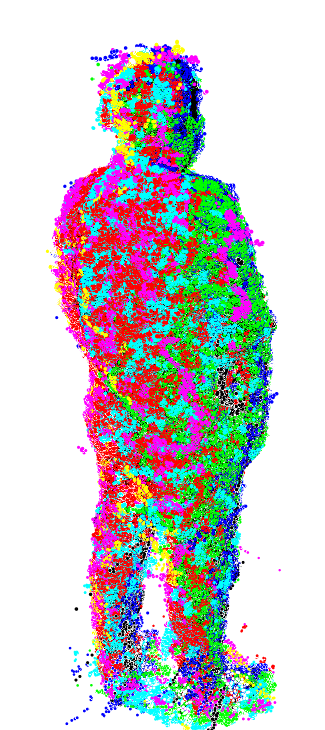
\includegraphics[width=2.5cm]{image/pc_4.png}
\end{minipage}
}
\caption{The reconstruction results of the back of a human using various methods. (a) results by Kalibr~\cite{Maye2013Self}, (b) results by Kalibr~\cite{Maye2013Self} with our registration step, (c) results by our global calibration method, (d) results by our integrated method. We render the point clouds with different colors to distinguish which view the point clouds belong to. The point clouds in result (a) are distinctly separated from other views, as the pink and green views cover the whole surface of the model. Result (b) becomes a little better while the green view still covers the right side of the body. The point clouds align quite well in result (c) with small blemishes, the azure view is inside the model. (d) shows a well-aligned model. }
\label{fig:pointcloud}
\end{figure*}


\begin{figure*}[htbp]
  \centering
\subfigure[]{
\begin{minipage}[c]{.22\linewidth}
\centering
  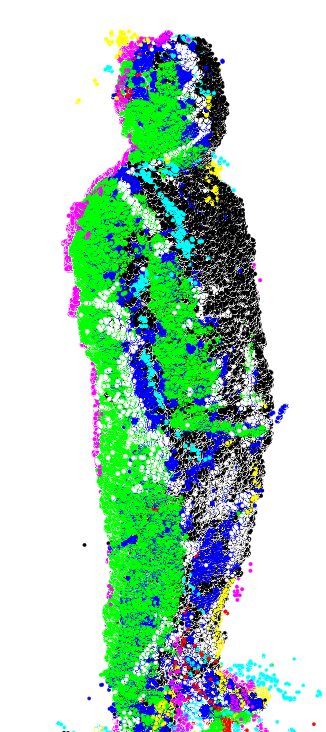
\includegraphics[width=2.6cm]{image/pc_1_1.png}
\end{minipage}
}%
\subfigure[]{
\begin{minipage}[c]{.22\linewidth}
\centering
  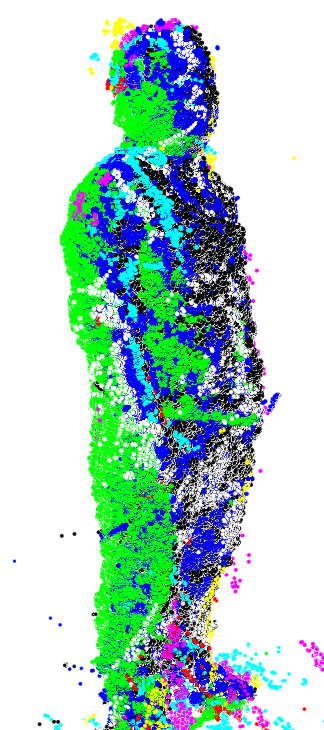
\includegraphics[width=2.6cm]{image/pc_2_1.png}
\end{minipage}
}
\subfigure[]{
\begin{minipage}[c]{.22\linewidth}
\centering
  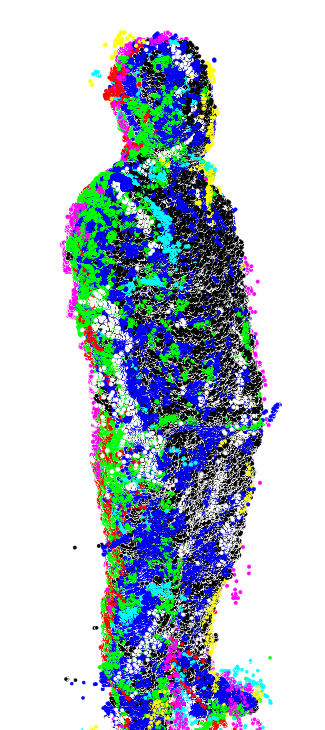
\includegraphics[width=2.6cm]{image/pc_3_1.png}
\end{minipage}
}
\subfigure[]{
\begin{minipage}[c]{.22\linewidth}
\centering
  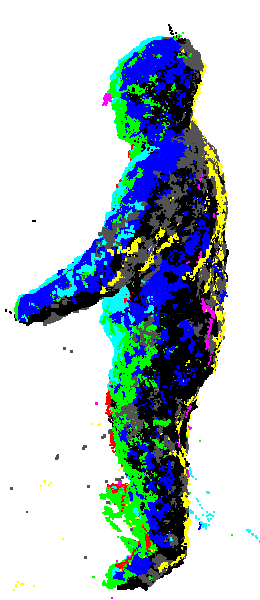
\includegraphics[width=2.6cm]{image/pc_4_1.png}
\end{minipage}
}
\caption{The reconstruction results of the left side of a human using various methods. (a) results by Kalibr~\cite{Maye2013Self}, (b) results by Kalibr~\cite{Maye2013Self} with our registration step, (c) results by our global calibration method, (d) results by our integrated method. The grey view in result (a) covers the surface and the black view is nearly inside the model especially on the shoulders and arms. Result (b) becomes a little better in black and grey view, however the green view covers the front of the model. There are similar problems in result (c), as the blue view covers the surface of the arm and head. Result (d) shows a well-aligned model, especially for the leg and arm with less separation between different views.}
\label{fig:pointcloud1}
\end{figure*}

\begin{figure*}[htbp]
  \centering
\subfigure[]{
\begin{minipage}[c]{.22\linewidth}
\centering
  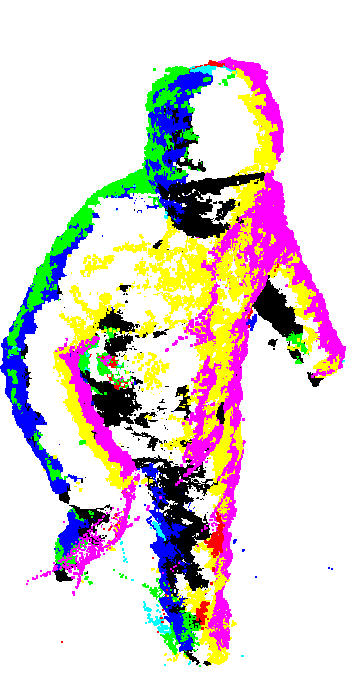
\includegraphics[width=2.5cm]{image/pc_1_2.png}
\end{minipage}
}%
\subfigure[]{
\begin{minipage}[c]{.22\linewidth}
\centering
  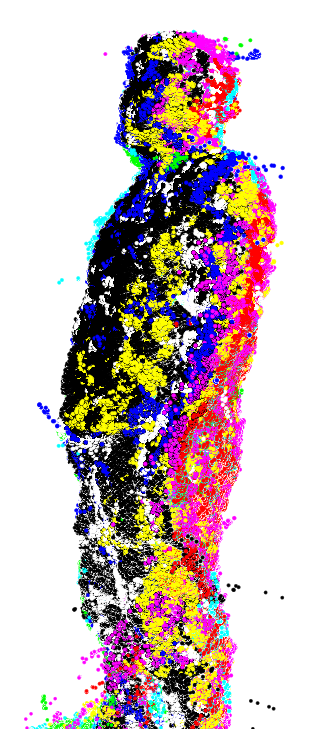
\includegraphics[width=2.5cm]{image/pc_2_2.png}
\end{minipage}
}
\subfigure[]{
\begin{minipage}[c]{.22\linewidth}
\centering
  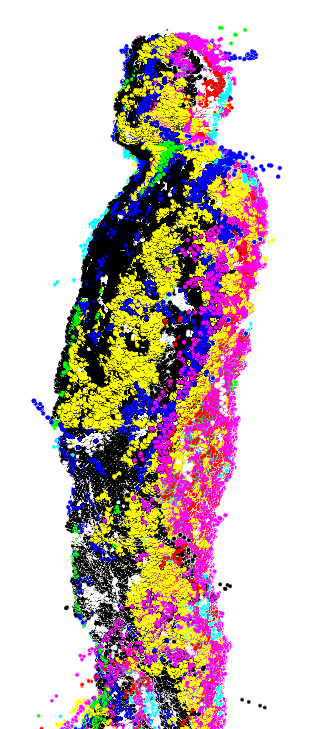
\includegraphics[width=2.5cm]{image/pc_3_2.png}
\end{minipage}
}
\subfigure[]{
\begin{minipage}[c]{.22\linewidth}
\centering
  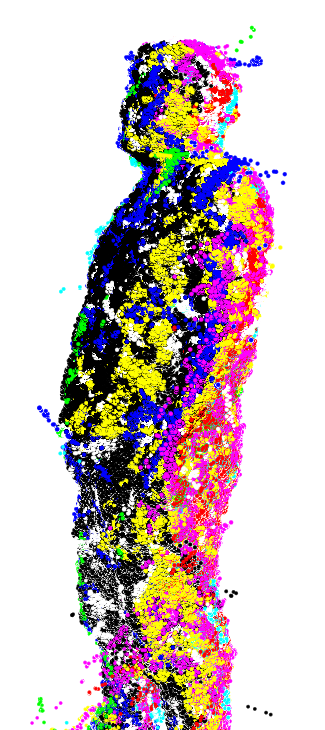
\includegraphics[width=2.5cm]{image/pc_4_2.png}
\end{minipage}
}
\caption{The reconstruction results of the front of a human using various methods. (a) results by Kalibr~\cite{Maye2013Self}, (b) results by Kalibr~\cite{Maye2013Self} with our registration step, (c) results by our global calibration method, (d) results by our integrated method. The white view covers the most surface of the right arm and the right chest, meanwhile the black view is inside the model in result (a).  The point clouds align a little well in result (b), however the yellow view covers the left side of the body, and the blue view is nearly covered by other views. On the contrary, the blue view covers the right side of the body in result (c), especially on the arm and the shoulder. The point clouds more or less separated from other views in these results, while (d) shows a well-aligned model.}
\label{fig:pointcloud2}
\end{figure*}
We reconstruct the 3D point clouds of a human body standing in our multi-camera system using various methods.  We mark the point cloud in different views with different colors to show the quality of the fusion results. Figure~\ref{fig:pointcloud}, ~\ref{fig:pointcloud1} and ~\ref{fig:pointcloud2} show the results in different human pose which demonstrate our algorithm. As we can see, the model reconstructed by our hybrid system has the highest quality.


\section{conclusion}
We present an efficient system integrating the multi-camera calibration and point cloud registration. By a global bundle adjustment, we reduce the accumulative error and the inconsistence caused by the pairwise camera pose estimation, and achieve a set of accurate extrinsic parameters with less reprojection error. With the point cloud registration, we minimize the error from the depth estimation and achieve a high-quality 3D model. Our calibration algorithm has been tested on both reprojection error and ground truth data. The experimental results has proved that the two steps of our system are both necessary and effective, and a more accuracy model can be reconstructed using our method.



